\chapter{Литературный обзор} \label{chapt1}


Для описания электронной структуры кристаллов или кристаллических 
поверхностей, обладающих пространственной периодичностью используется
зонная модель~\cite{Kittel1976}. В общем случае задача об электронах 
твердого тела является многоэлектронной задачей, потому что полный 
гамильтониан в твердых телах содержит не только одноэлектронные 
потенциалы, описывающие взаимодействие легкого электрона с массивным 
ядром, но и потенциалы взаимодействия электронов между собой~\cite{Simonov_disser}.
В приближении свободных электронов такое взаимодействие описывается
с помощью эффективного одноэлектронного потенциала $U(\vec{r})$. 
Вне зависимости от формы этого потенциала, для идеального периодического
кристалла он будет удовлетворять условию периодичности:
\begin{equation}
	\label{one_electron_potential}
	U(\vec{r})=U(\vec{r}+\vec{R})
\end{equation}
для всех векторов $\vec{R}$, принадлежащих решетке Браве.


В рамках одноэлектронной модели движение электрона в кристалле описывается
уравнением Шредингера:
\begin{equation}
	\label{Shredinger_equation}
	H\psi=\left(\frac{-\hbar^2}{2m}\Delta+U(\vec{r})\right)\psi=\varepsilon\psi
\end{equation}
где $U(\vec{r})$ - эффективный потенциал, удовлетворяющий условию~\ref{one_electron_potential}.


Следствием периодичности потенциала является очень важное свойство 
стационарных состояний - теорема Блоха. Согласно этой теореме 
собственные состояния оператора \textit{H} можно выбрать таким образом,
чтобы с каждым из них был связан некоторый волновой вектор $\vec{k}$ и 
для любого $\vec{R}$ в решетке Браве выполнялось равенство:
\begin{equation}
	\label{equaliation_of_wave_func}
	\psi(\vec{r}+\vec{R})=e^{i\vec{k}\vec{R}}\psi(\vec{r})
\end{equation}


При этом $\psi(\vec{r})$ представима в виде Блоховской волны:
\begin{equation}
	\label{Bloh_wave}
	\psi(\vec{r})=e^{i\vec{k}\vec{R}}u(\vec{r})
\end{equation}
где
\begin{equation}
	\label{u_wave}
	u(\vec{r}+\vec{R})=u(\vec{r})
\end{equation}


Введенный вектор $\vec{k}$ является квантовым числом, которое 
характеризует трансляционную симметрию периодического потенциала. 
В общей задаче о движении в периодическом потенциале он играет ту же роль, что и волновой вектор $\vec{k}$ свободного электрона в теории 
Зоммерфельда~\cite{Kittel1976}. Однако, нужно заметить, что в отличие 
от состояний свободного электрона, в периодическом потенциале одно
и то же состояние электрона характеризуется бесконечным набором векторов
$\vec{k}, \vec{k'}, \vec{k''}$ и т. д., отличающихся друг от друга на вектор $\vec{K}$ обратной решетки (см.~\ref{equaliation_of_wave_func}).
По этой причине вектор $\vec{k}$ называют квазиволновым вектором, а
$\hbar\vec{k}$ - соответствующим квазиимпульсом. Так как для двух
значений $\vec{k}$, отличающихся друг от друга на вектор обратной 
решетки, все волновые функции и энергетические уровни совпадают,
для полного описания всей совокупности уровней достаточно ограничить
область значений $\vec{k}$ одной элементарной ячейкой.
Зоной Бриллюэна называют область обратного пространства, которое включает
в себя все множество неэквивалентных значений квазиволнового вектора.
Для обратной решетки первая зона Бриллюэна совпадает с ячейкой 
Вигнера-Зейтца~\cite{Kittel1976}. По теореме Блоха можно показать, что 
энергетические уровни электрона в периодическом потенциале могут быть описаны с помощью непрерывных функций $\varepsilon_n(\vec{k})$(\textit{n} - 
номер энергетической зоны), каждая из которых имеет периодичность
обратной решетки. Структуру твердого тела определяют именно эти 
функции\cite{Simonov_disser}.
\begin{figure}[!ht]
\center{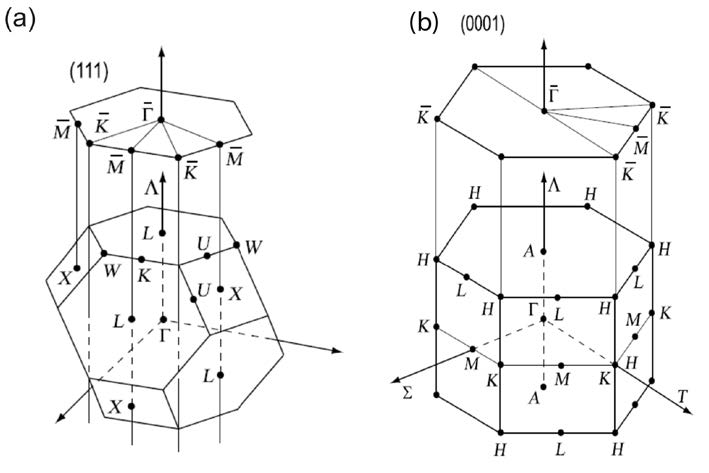
\includegraphics[width=0.7\linewidth]{zones.png}}
\caption{Связь между двумерной зоной Бриллюэна плоскости(111) fcc
кристалла (a), плоскости (0001) гексагонального кристалла (b) и 
объемной зоной Бриллюэна~\cite{Hufner2019}}
\label{pic:Brilluen_zones}
\end{figure}


Для анализа систем с пространственной периодичностью концепция
зон Бриллюэна играет очень важную роль. На рис.~\ref{pic:Brilluen_zones}
показаны двумерные зоны Бриллюэна для плотноупакованной грани (111) 
гранецентрированного кубического (fcc) кристалла и грани (0001)
гексагонального кристалла. Так же на этом рисунке показана связь с 
объемными Зонами Бриллюэна~\cite{Hufner2019}. 




\section{Двумерные структуры} \label{sect1_1}